\begin{frame}
    \frametitle{$k$ Nearest Neighbor}
    \begin{itemize}
        \item Classification: same setup as logistic regression.
        \item Very simple but powerful idea: Do as your neighbors does.
        \item For a new point $x$ look at the nearest (or the two nearest or three nearest, \ldots)
            point in the training data for a label.
        \item Usually: Euclidean distance in $\mathbb{R}^d$
    \end{itemize}
\end{frame}

\begin{frame}
    \frametitle{Simple algorithm}
    \begin{itemize}
        \item Pick a $k$, for example $k=3$.
        \item Want to classify new example $x$.
        \item Compute $d_i = d(x_i, x)$, i.e.\, $d(x_i, x) = ||x_i - x||$
        \item Sort $d_i$, take $k$ smallest: $d_{i_0}, d_{i_1}, d_{i_2}$.
        \item Assign $y$ that appears most often among $y_{i_0}, y_{i_1}, y_{i_2}$
    \end{itemize}
\end{frame}

\begin{frame}
    \frametitle{Illustration}
    \begin{center}
    \includegraphics<1>[width=.6\linewidth]{knn-pics/two_moons}
    \includegraphics<2>[width=.6\linewidth]{knn-pics/two_moons_k=5}
    \end{center}
\end{frame}

\begin{frame}
    \frametitle{Picking $k$}
    \begin{itemize}
        \item General problem called model selection.
        %\item Model selection is necessary for nearly all algorithms.
        \item For training data, $k=1$ gives perfect prediction -- but not for new data!
        %\item Larger $k$ leads to smoother boundaries and worse performance on the training set,
            %but better on the test set.
    \end{itemize}
    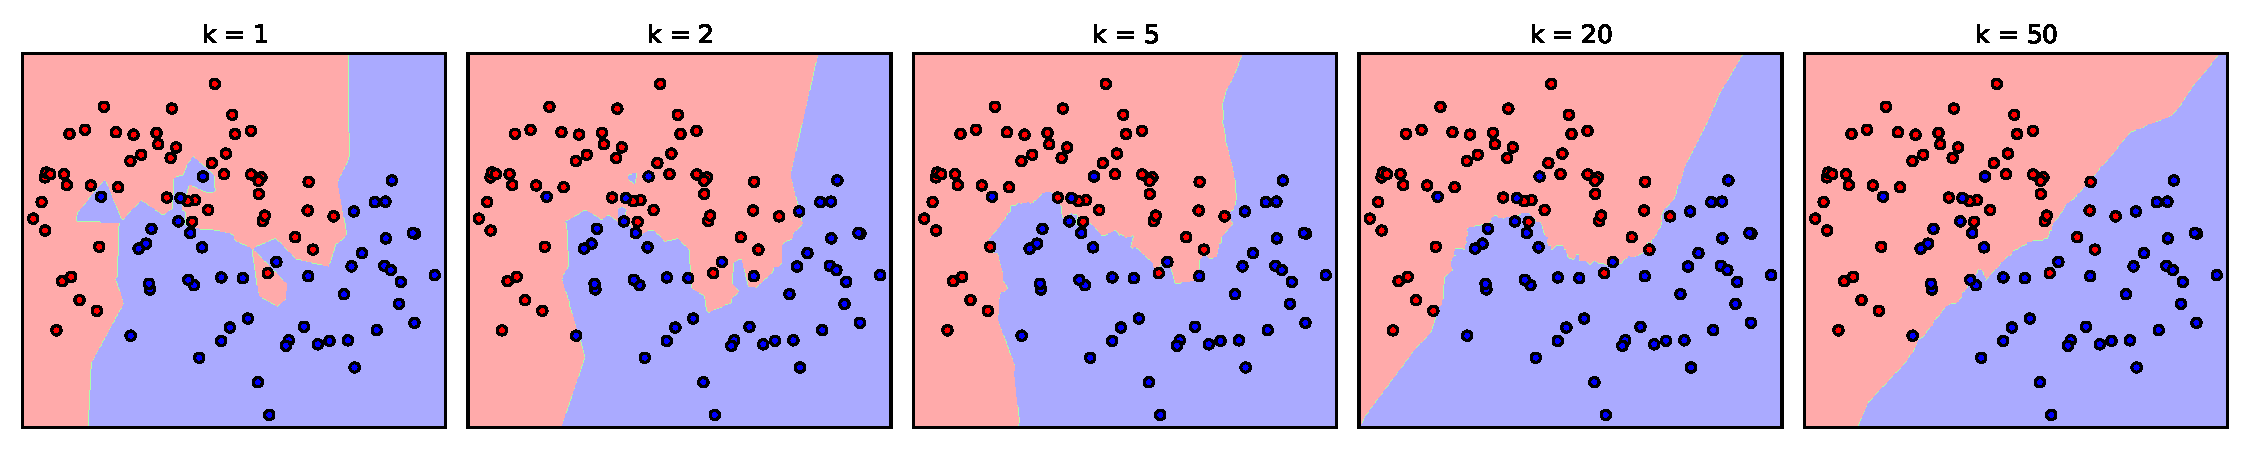
\includegraphics[width=.98\linewidth]{knn-pics/two_moons_varying_k}
\end{frame}


\begin{frame}[t]
    \frametitle{Really: Picking $k$ (in practice)}
    \begin{itemize}
        \item We can not choose $k$ on the training set.
        \item We can not choose $k$ on the set we evaluate our algorithm on (or
            for that we need predictions).
    \end{itemize}
    \center
        \begin{onlyenv}<2>
            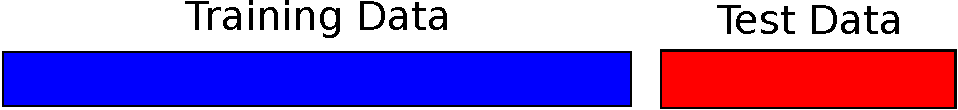
\includegraphics[width=.7\linewidth]{knn-pics/train_test_bars-crop}\\
        \end{onlyenv}
        \begin{onlyenv}<3->
            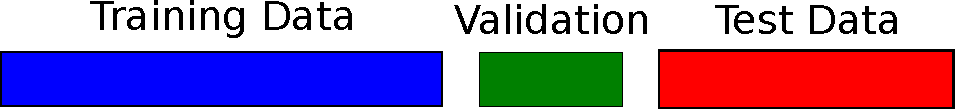
\includegraphics[width=.7\linewidth]{knn-pics/train_val_test_bars-crop}\\
        \end{onlyenv}

    \includegraphics<4>[width=.7\linewidth]{knn-pics/two_moons_cross_validation_1}
    \includegraphics<5>[width=.7\linewidth]{knn-pics/two_moons_cross_validation_2}
    \includegraphics<6>[width=.7\linewidth]{knn-pics/two_moons_cross_validation_3}

\end{frame}

%\begin{frame}
    %\frametitle{$k$ Nearest Neighbor -- Interactive}
    %\begin{itemize}
        %\item  start with blobs from k-means
        %\item  Iris dataset
        %\item  Measure prediction error
        %\item  Maybe: Complexity curve visualization (needs a loop)
    %\end{itemize}
%\end{frame}
